\begin{frame}{XGBoost pour la Régression : Initialisation}
    \begin{columns}[T]
        \begin{column}{0.42\textwidth}
            \textbf{Jeu de données (Médicaments) :}
            
            \begin{table}
                \centering
                \scriptsize
                \begin{tabular}{|c|c|}
                    \hline
                    \textbf{Dosage (mg)} & \textbf{Efficacité} \\
                    \hline
                    10 & -10 \\
                    20 & 7 \\
                    25 & 8 \\
                    35 & -7 \\
                    \hline
                \end{tabular}
            \end{table}
            
            \begin{block}{Prédiction initiale $f_0(x)$}
                \scriptsize
                Valeur par défaut : \textbf{0.5}.
                
                \textbf{Pourquoi 0.5 ?} \\
                Dans XGBoost, le score de base (\texttt{base\_score}) est initialisé à 0.5 par défaut, un héritage de la probabilité. En régression, ce "décalage" n'est pas pénalisant : les arbres de gradient vont très vite corriger cette valeur initiale via l'apprentissage itératif des résidus.
            \end{block}
        \end{column}
        
        \begin{column}{0.58\textwidth}
            \begin{center}
            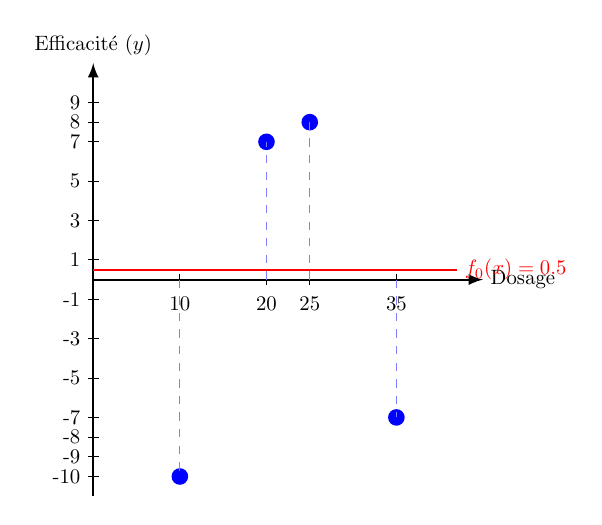
\begin{tikzpicture}[x=0.11cm, y=0.25cm, every node/.style={scale=0.75}]
                % Axes
                \draw[->, thick, -latex] (0,-11) -- (0,11) node[above] {Efficacité ($y$)};
                \draw[->, thick, -latex] (0,0) -- (45,0) node[right] {Dosage};
                
                % Ticks sur l'axe Y
                \foreach \y in {-10, -9,-8,-7, -5, -3, -1, 1, 3, 5, 7, 8, 9} {
                    \draw (2pt,\y) -- (-2pt,\y) node[left] {\y};
                }
                
                % Ticks sur l'axe X
                \foreach \x in {10, 20, 25, 35} {
                    \draw (\x, 2pt) -- (\x, -2pt) node[below=2pt] {\x};
                }
                
                % Points de données
                \fill[blue] (10,-10) circle (3pt);
                \fill[blue] (20,7) circle (3pt);
                \fill[blue] (25,8) circle (3pt);
                \fill[blue] (35,-7) circle (3pt);
                
                % Ligne de prédiction initiale 0.5
                \draw[thick, red] (0, 0.5) -- (42, 0.5) node[right] {$f_0(x) = 0.5$};
                
                % Projection des points vers l'axe x
                \draw[dashed, blue!50] (10,0) -- (10,-10);
                \draw[dashed, blue!50] (20,0) -- (20,7);
                \draw[dashed, blue!50] (25,0) -- (25,8);
                \draw[dashed, blue!50] (35,0) -- (35,-7);

            \end{tikzpicture}
            \end{center}
        \end{column}
    \end{columns}
\end{frame}

% Frame 2 : Résidus et Formules
\begin{frame}{XGBoost pour la Régression : Résidus et Formules}
    \begin{columns}[T]
        \begin{column}{0.4\textwidth}
            \textbf{Calcul des Résidus ($r_i$) :} \\
            $r_i = y_i - f_0(x_i)$ \\
            \scriptsize (\textit{Efficacité réelle - prédiction})
            \vspace{0.1cm}
            
            \begin{table}
                \centering
                \scriptsize
                \begin{tabular}{|c|c|c|}
                    \hline
                    \textbf{Dosage} & \textbf{Effic.} & \textbf{Résidu ($r_i$)} \\
                    \hline
                    10 & -10 & \textbf{-10.5} \\
                    20 & 7 & \textbf{6.5} \\
                    25 & 8 & \textbf{7.5} \\
                    35 & -7 & \textbf{-7.5} \\
                    \hline
                \end{tabular}
            \end{table}
            
            \vspace{0.2cm}
            \scriptsize
            \textit{Exemple pour dosage 10 :} \\
            $r_1 = -10 - 0.5 = -10.5$
        \end{column}
        
        \begin{column}{0.6\textwidth}
            \begin{block}{Métriques de construction}
                \scriptsize
                \textbf{1. Similarity Score (SS) :}
                $ SS = \frac{(\sum \text{Résidus})^2}{\text{Nb. Résidus} + \lambda} $ \\
                \textit{Évalue la pureté du nœud.}
                
                \textbf{2. Gain :} 
                $ Gain = SS_{gauche} + SS_{droit} - SS_{racine} - \gamma $ \\
                \textit{Mesure l'amélioration apportée par l'embranchement.}
                
                \textbf{3. Hyperparamètres de Régularisation :}
                \begin{itemize}
                    \setlength\itemsep{0em}
                    \item $\lambda$ (Lambda) : Régularisation L2. Diminue l'influence des observations individuelles.
                    \item $\gamma$ (Gamma) : Seuil minimal de Gain requis pour diviser.
                \end{itemize}
            \end{block}
         
            \scriptsize
            \textbf{Score de la Racine} (avec $\lambda=0$) : \\
            Somme des résidus = -4. Nombre = 4. \\
            $\rightarrow SS_{racine} = \frac{(-4)^2}{4+0} = \frac{16}{4} = 4$.
        \end{column}
    \end{columns}
\end{frame}

% Frame 3 : Splits 1 et 2
\begin{frame}{XGBoost : Évaluation des Splits (Arbre 1)}
    \vspace{-0.2cm}
    \textit{\small On évalue les moyennes entre dosages consécutifs : 15, 22.5, 30. ($\lambda=0, \gamma=0$)}
    
    \begin{columns}[T]
        % SPLIT 1
        \begin{column}{0.5\textwidth}
            \begin{block}{Split 1 : Dosage < 15}
                \centering
                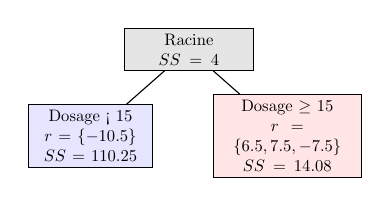
\begin{tikzpicture}[every node/.style={scale=0.6}, level/.style={sibling distance=2.5cm, level distance=1.1cm}]
                    \node[draw, rectangle, fill=gray!20, text width=2.5cm, align=center] {Racine \\ $SS = 4$}
                        child {node[draw, rectangle, fill=blue!10, text width=2.4cm, align=center] {Dosage < 15 \\ $r=\{-10.5\}$ \\ $SS = 110.25$}}
                        child {node[draw, rectangle, fill=red!10, text width=2.9cm, align=center] {Dosage $\geq$ 15 \\ $r=\{6.5, 7.5, -7.5\}$ \\ $SS = 14.08$}};
                \end{tikzpicture}
                \vspace{0.1cm}
                
                \footnotesize \textbf{Gain} $= 110.25 + 14.08 - 4 = \textbf{120.33}$
                
                \vspace{0.1cm}
                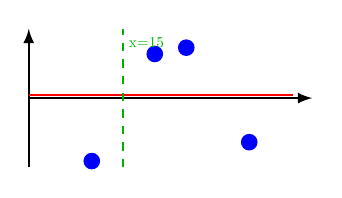
\begin{tikzpicture}[x=0.08cm, y=0.08cm, every node/.style={scale=0.55}]
                    \draw[->, thick, -latex] (0,-11) -- (0,11);
                    \draw[->, thick, -latex] (0,0) -- (45,0);
                    \fill[blue] (10,-10) circle (3pt); \fill[blue] (20,7) circle (3pt);
                    \fill[blue] (25,8) circle (3pt); \fill[blue] (35,-7) circle (3pt);
                    \draw[thick, red] (0, 0.5) -- (42, 0.5);
                    \draw[thick, green!70!black, dashed] (15, -11) -- (15, 11) node[pos=0.9, right] {x=15};
                \end{tikzpicture}
            \end{block}
        \end{column}
        
        % SPLIT 2
        \begin{column}{0.5\textwidth}
            \begin{block}{Split 2 : Dosage < 22.5}
                \centering
                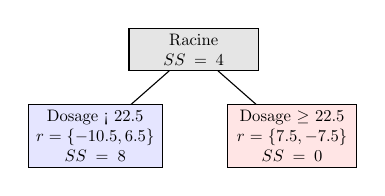
\begin{tikzpicture}[every node/.style={scale=0.6}, level/.style={sibling distance=2.5cm, level distance=1.1cm}]
                    \node[draw, rectangle, fill=gray!20, text width=2.5cm, align=center] {Racine \\ $SS = 4$}
                        child {node[draw, rectangle, fill=blue!10, text width=2.6cm, align=center] {Dosage < 22.5 \\ $r=\{-10.5, 6.5\}$ \\ $SS = 8$}}
                        child {node[draw, rectangle, fill=red!10, text width=2.5cm, align=center] {Dosage $\geq$ 22.5 \\ $r=\{7.5, -7.5\}$ \\ $SS = 0$}};
                \end{tikzpicture}
                \vspace{0.1cm}
                
                \footnotesize \textbf{Gain} $= 8 + 0 - 4 = \textbf{4.00}$
                
                \vspace{0.1cm}
                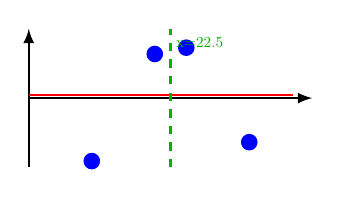
\begin{tikzpicture}[x=0.08cm, y=0.08cm, every node/.style={scale=0.55}]
                    \draw[->, thick, -latex] (0,-11) -- (0,11);
                    \draw[->, thick, -latex] (0,0) -- (45,0);
                    \fill[blue] (10,-10) circle (3pt); \fill[blue] (20,7) circle (3pt);
                    \fill[blue] (25,8) circle (3pt); \fill[blue] (35,-7) circle (3pt);
                    \draw[thick, red] (0, 0.5) -- (42, 0.5);
                    \draw[thick, green!70!black, dashed] (22.5, -11) -- (22.5, 11) node[pos=0.9, right] {x=22.5};
                \end{tikzpicture}
            \end{block}
        \end{column}
    \end{columns}
\end{frame}

% Frame 4 : Split 3 et Conclusion
\begin{frame}{XGBoost : Split 3 et Conclusion de l'Arbre 1}
    \begin{columns}[T]
        % SPLIT 3
        \begin{column}{0.5\textwidth}
            \begin{block}{Split 3 : Dosage < 30}
                \centering
                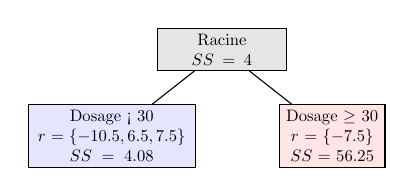
\begin{tikzpicture}[every node/.style={scale=0.6}, level/.style={sibling distance=2.8cm, level distance=1.1cm}]
                    \node[draw, rectangle, fill=gray!20, text width=2.5cm, align=center] {Racine \\ $SS = 4$}
                        child {node[draw, rectangle, fill=blue!10, text width=3.3cm, align=center] {Dosage < 30 \\ $r=\{-10.5, 6.5, 7.5\}$ \\ $SS = 4.08$}}
                        child {node[draw, rectangle, fill=red!10, text width=2.0cm, align=center] {Dosage $\geq$ 30 \\ $r=\{-7.5\}$ \\ $SS = 56.25$}};
                \end{tikzpicture}
                \vspace{0.1cm}
                
                \footnotesize \textbf{Gain} $= 4.08 + 56.25 - 4 = \textbf{56.33}$
                
                \vspace{0.1cm}
                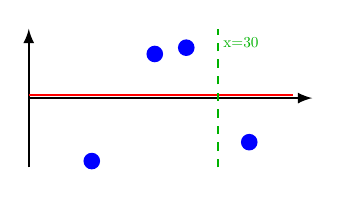
\begin{tikzpicture}[x=0.08cm, y=0.08cm, every node/.style={scale=0.55}]
                    \draw[->, thick, -latex] (0,-11) -- (0,11);
                    \draw[->, thick, -latex] (0,0) -- (45,0);
                    \fill[blue] (10,-10) circle (3pt); \fill[blue] (20,7) circle (3pt);
                    \fill[blue] (25,8) circle (3pt); \fill[blue] (35,-7) circle (3pt);
                    \draw[thick, red] (0, 0.5) -- (42, 0.5);
                    \draw[thick, green!70!black, dashed] (30, -11) -- (30, 11) node[pos=0.9, right] {x=30};
                \end{tikzpicture}
            \end{block}
        \end{column}
        
        % VERDICT
        \begin{column}{0.5\textwidth}
            \begin{block}{Comparaison des Splits ($\lambda=0, \gamma=0$)}
                \scriptsize
                \begin{itemize}
                    \setlength\itemsep{0em}
                    \item Gain (Split < 15) : \textbf{120.33}
                    \item Gain (< 22.5) : 4.00 \quad | \quad Gain (< 30) : 56.33
                \end{itemize}
            \end{block}
            
            \begin{block}{Verdict de l'algorithme}
                \scriptsize
                L'approche gloutonne (Greedy Algorithm) sélectionne le split \textbf{maximisant le Gain}.
                
                $\Rightarrow$ On isole la valeur très négative en coupant à \textbf{Dosage < 15}.
                
                \vspace{0.1cm}
                \tiny \textit{Le processus se répète ensuite de façon récursive sur les nœuds enfants.}
            \end{block}
        \end{column}
    \end{columns}
\end{frame}

% Frame 5 : Poursuite de l'arbre
\begin{frame}{XGBoost : Poursuite de la construction (Nœud Droit)}
    \vspace{-0.2cm}
    \textit{\small Le nœud de droite (Dosage $\geq$ 15) contient les résidus \{6.5, 7.5, -7.5\}. Coupures possibles : 22.5 et 30.}
    
    \begin{columns}[T]
        % NOUVEAUX SPLITS
        \begin{column}{0.5\textwidth}
            \begin{block}{Nouvelle coupure : < 22.5}
                \centering
                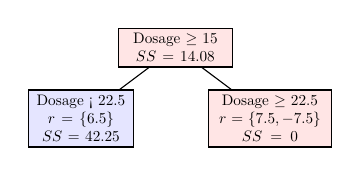
\begin{tikzpicture}[every node/.style={scale=0.55}, level/.style={sibling distance=2.4cm, level distance=0.9cm}]
                    \node[draw, rectangle, fill=red!10, text width=2.4cm, align=center] {Dosage $\geq$ 15 \\ $SS = 14.08$}
                        child {node[draw, rectangle, fill=blue!10, text width=2.2cm, align=center] {Dosage < 22.5 \\ $r=\{6.5\}$ \\ $SS = 42.25$}}
                        child {node[draw, rectangle, fill=red!10, text width=2.6cm, align=center] {Dosage $\geq$ 22.5 \\ $r=\{7.5, -7.5\}$ \\ $SS = 0$}};
                \end{tikzpicture}
                
                \scriptsize \textbf{Gain} $= 42.25 + 0 - 14.08 = \textbf{28.17}$
            \end{block}
            
            \begin{block}{Nouvelle coupure : < 30}
                \centering
                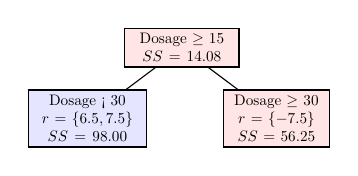
\begin{tikzpicture}[every node/.style={scale=0.55}, level/.style={sibling distance=2.4cm, level distance=0.9cm}]
                    \node[draw, rectangle, fill=red!10, text width=2.4cm, align=center] {Dosage $\geq$ 15 \\ $SS = 14.08$}
                        child {node[draw, rectangle, fill=blue!10, text width=2.5cm, align=center] {Dosage < 30 \\ $r=\{6.5, 7.5\}$ \\ $SS = 98.00$}}
                        child {node[draw, rectangle, fill=red!10, text width=2.2cm, align=center] {Dosage $\geq$ 30 \\ $r=\{-7.5\}$ \\ $SS = 56.25$}};
                \end{tikzpicture}
                
                \scriptsize \textbf{Gain} $= 98.00 + 56.25 - 14.08 = \textbf{140.17}$
            \end{block}
        \end{column}
        
        % ARBRE FINAL & SORTIE
        \begin{column}{0.5\textwidth}
            \begin{block}{Arbre final (Profondeur = 2)}
                \centering
                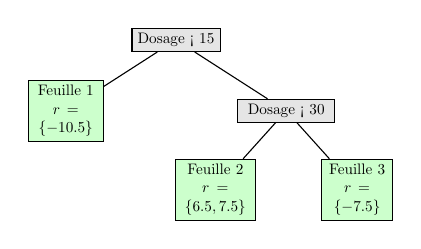
\begin{tikzpicture}[every node/.style={scale=0.55}, level 1/.style={sibling distance=2.8cm, level distance=0.9cm}, level 2/.style={sibling distance=1.8cm, level distance=1cm}]
                    \node[draw, rectangle, fill=gray!20, text width=1.8cm, align=center] {Dosage < 15}
                        child {node[draw, rectangle, fill=green!20, text width=1.5cm, align=center] {Feuille 1 \\ $r=\{-10.5\}$}}
                        child {node[draw, rectangle, fill=gray!20, text width=2.0cm, align=center] {Dosage < 30}
                            child {node[draw, rectangle, fill=green!20, text width=1.6cm, align=center] {Feuille 2 \\ $r=\{6.5, 7.5\}$}}
                            child {node[draw, rectangle, fill=green!20, text width=1.4cm, align=center] {Feuille 3 \\ $r=\{-7.5\}$}}
                        };
                \end{tikzpicture}
            \end{block}
            
            \begin{block}{Valeurs de Sortie (Output)}
                \scriptsize
                Pour chaque feuille, on calcule la valeur de sortie :
                $\text{Output} = \frac{\sum \text{Résidus}}{\text{Nb. Résidus} + \lambda}$
                
                \begin{itemize}
                    \setlength\itemsep{0em}
                    \item F1 : $-10.5 / 1 = \textbf{-10.5}$
                    \item F2 : $(6.5+7.5)/2 = \text{14} / 2 = \textbf{7}$
                    \item F3 : $-7.5 / 1 = \textbf{-7.5}$
                \end{itemize}
            \end{block}
        \end{column}
    \end{columns}
\end{frame}

% Frame 6 : Effet de Lambda et Gamma
\begin{frame}{XGBoost : Régularisation par $\lambda$ et $\gamma$}
    \vspace{-0.2cm}
    \begin{block}{1. Effet de Lambda ($\lambda$) sur le Score de Similarité}
        \scriptsize $SS = \frac{(\sum \text{Résidus})^2}{N + \lambda}$ \quad ($N$ = nombre d'obs.). Si $\lambda>0$, le $SS$ baisse.
        
        \textbf{Réduction inversement proportionnelle à $N$} :
        \begin{itemize}
            \setlength\itemsep{0em}
            \item \textbf{Peu de données} ($N=1$) : $\lambda$ domine le dénominateur $\rightarrow$ baisse \textbf{drastique} du $SS$.
            \item \textbf{Beaucoup de données} ($N=100$) : l'ajout de $\lambda$ devient négligeable.
        \end{itemize}
        $\Rightarrow$ \textbf{Effet :} $\lambda$ pénalise le surapprentissage en élaguant les feuilles très isolées.
    \end{block}

    \begin{columns}[T]
        \begin{column}{0.5\textwidth}
            \begin{block}{Exemple comparatif ($SS$ avec $\lambda=1$)}
                \scriptsize
                \textbf{Feuille isolée ($N=1$, R=$7.5$)} :
                \begin{itemize}
                    \setlength\itemsep{0em}
                    \item $\lambda=0 \rightarrow SS = 7.5^2 / 1 = \textbf{56.25}$
                    \item $\lambda=1 \rightarrow SS = 7.5^2 / 2 = \textbf{28.12}$ {\color{red} (-50\%)}
                \end{itemize}
                
                \textbf{Feuille groupée ($N=2$, R=$6.5, 7.5$)} :
                \begin{itemize}
                    \setlength\itemsep{0em}
                    \item $\lambda=0 \rightarrow SS = 14^2 / 2 = \textbf{98.00}$
                    \item $\lambda=1 \rightarrow SS = 14^2 / 3 = \textbf{65.33}$ {\color{red} (-33\%)}
                \end{itemize}
            \end{block}
        \end{column}
        
        \begin{column}{0.5\textwidth}
            \begin{block}{2. Effet de Gamma ($\gamma$)}
                \scriptsize
                $Gain = SS_{gauche} + SS_{droit} - SS_{racine} - \gamma$
                
                \vspace{0.1cm}
                Élagage de bas en haut (Post-Pruning) :
                \begin{itemize}
                    \setlength\itemsep{0em}
                    \item Si \textbf{Gain < 0}, la branche est supprimée.
                    \item $\gamma$ représente un seuil de "péage" minimal.
                \end{itemize}
                \vspace{0.1cm}
                $\Rightarrow$ \textbf{Effet :} $\gamma$ exige une amélioration \textbf{substantielle}, évitant de conserver les ajustements microscopiques du modèle.
            \end{block}
        \end{column}
    \end{columns}
\end{frame}

% Frame 7 : Learning Rate et Nouvelles Prédictions
\begin{frame}{XGBoost : Application du Learning Rate ($\eta$)}
    \begin{block}{Le Taux d'Apprentissage ($\eta$) / Shrinkage}
        Pour éviter le surapprentissage, la sortie de l'arbre n'est pas ajoutée intégralement. On applique une technique de \textbf{Shrinkage} (réduction) en multipliant par un taux $\eta$ (ex: $0.3$).
        
        \vspace{0.1cm}
        $$ f_1(x) = f_0(x) + \, \eta \, \times \text{Sortie Arbre}_1(x) $$
    \end{block}

    \begin{block}{Calcul des nouvelles prédictions et résidus}
        \centering
        \small
        \begin{tabular}{|c|c|c|c|}
            \hline
            \textbf{Dosage} & \textbf{Sortie Arbre} & \textbf{Nouvelle Préd. ($f_1$)} & \textbf{Nouveau Résidu ($r_i$)} \\
            \hline
            10 & -10.5 & $0.5 + 0.3(-10.5) = \textbf{-2.65}$ & $-10 - (-2.65) = \textbf{-7.35}$ \\
            \hline
            20 & 7 & $0.5 + 0.3(7) = \textbf{2.6}$ & $7 - 2.6 = \textbf{4.4}$ \\
            \hline
            25 & 7 & $0.5 + 0.3(7) = \textbf{2.6}$ & $8 - 2.6 = \textbf{5.4}$ \\
            \hline
            35 & -7.5 & $0.5 + 0.3(-7.5) = \textbf{-1.75}$ & $-7 - (-1.75) = \textbf{-5.25}$ \\
            \hline
        \end{tabular}
    \end{block}
    
    \vspace{0.2cm}
    \textbf{Observation :} Tous les nouveaux résidus sont plus proches de 0 que les précédents (-10.5, 6.5, 7.5, -7.5). L'erreur globale a diminué !
\end{frame}

% Frame 8 : Visualisation et Itérations
\begin{frame}{XGBoost : Visualisation de $f_1(x)$ et Itérations}
    \begin{columns}[T]
        \begin{column}{0.55\textwidth}
            \centering
            \textbf{Un pas "prudent" vers la réalité ($\eta=0.3$)}
            
            \vspace{0.2cm}
            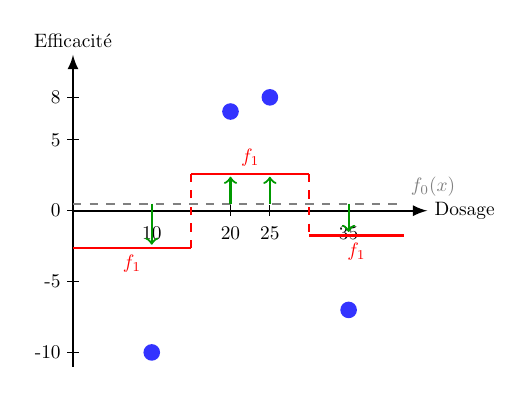
\begin{tikzpicture}[x=0.10cm, y=0.18cm, every node/.style={scale=0.7}]
                % Axes
                \draw[->, thick, -latex] (0,-11) -- (0,11) node[above] {Efficacité};
                \draw[->, thick, -latex] (0,0) -- (45,0) node[right] {Dosage};
                
                % Ticks sur l'axe Y
                \foreach \y in {-10, -5, 0, 5, 8} {
                    \draw (2pt,\y) -- (-2pt,\y) node[left] {\y};
                }
                \foreach \x in {10, 20, 25, 35} {
                    \draw (\x, 2pt) -- (\x, -2pt) node[below=2pt] {\x};
                }
                
                % Points de données réelles (Transparents)
                \fill[blue, opacity=0.8] (10,-10) circle (3pt);
                \fill[blue, opacity=0.8] (20,7) circle (3pt);
                \fill[blue, opacity=0.8] (25,8) circle (3pt);
                \fill[blue, opacity=0.8] (35,-7) circle (3pt);
                
                % f0(x)
                \draw[thick, gray, dashed] (0, 0.5) -- (42, 0.5) node[above right] {$f_0(x)$};
                
                % f1(x) par paliers
                \draw[thick, red] (0, -2.65) -- (15, -2.65) node[midway, below] {$f_1$};
                \draw[thick, red, dashed] (15, -2.65) -- (15, 2.6);
                \draw[thick, red] (15, 2.6) -- (30, 2.6) node[midway, above] {$f_1$};
                \draw[thick, red, dashed] (30, 2.6) -- (30, -1.75);
                \draw[thick, red] (30, -1.75) -- (42, -1.75) node[midway, below] {$f_1$};
                
                % Flèches montrant la réduction du résidu (de f0 à f1)
                \draw[->, green!60!black, thick] (10, 0.5) -- (10, -2.4); % direction -10
                \draw[->, green!60!black, thick] (20, 0.5) -- (20, 2.4);  % direction 7
                \draw[->, green!60!black, thick] (25, 0.5) -- (25, 2.4);  % direction 8
                \draw[->, green!60!black, thick] (35, 0.5) -- (35, -1.5); % direction -7
            \end{tikzpicture}
        \end{column}
        
        \begin{column}{0.45\textwidth}
            \begin{block}{La suite de l'algorithme}
                \scriptsize
                L'erreur diminue progressivement ("booster").
                
                \vspace{0.1cm}
                Désormais, pour l'étape suivante :
                \begin{itemize}
                    \setlength\itemsep{0em}
                    \item Construction de l'\textbf{Arbre 2}.
                    \item Cible : les \textbf{nouveaux résidus} $r_i$ qu'il nous reste à combler (-7.35, 4.4, 5.4, -5.25).
                \end{itemize}
                
                \vspace{0.1cm}
                Le processus se répète itérativement ($f_2, f_3, \dots, f_M$) jusqu'à :
                \begin{itemize}
                    \setlength\itemsep{0em}
                    \item Atteindre $M$ arbres (\texttt{n\_estimators}).
                    \item Erreur quasi-nulle (\textit{Early Stopping}).
                \end{itemize}
            \end{block}
        \end{column}
    \end{columns}
\end{frame}